\chapter*{Bijlagen}

\begin{tabular}{ll}

  

Bijlage A \textbf{(op SD)}  &	De CIF-dictionary 
\\ \\
Bijlage B: &	Cif-bestand van de kristalstructuur van Chaziet  
\\ \\
Bijlage C \textbf{(op SD)}: &	Zelf ontworpen CIF-parser
\\ \\
Bijlage D \textbf{(op SD)}: &	Volledige code van het programma 
\\ \\
Bijlage E : & Externe dictionary met stralen van elementen
\\ \\
Bijlage F : & Externe dictionary met kleuren van elementen
\\ \\
Bijlage G : & Specs van het gebruikte systeem
\\ \\
Bijlage H \textbf{(op SD)}:& ZIP bestand met daarin de add-on
\\ \\
\end{tabular}
\newpage

\chapter*{Bijlage B}
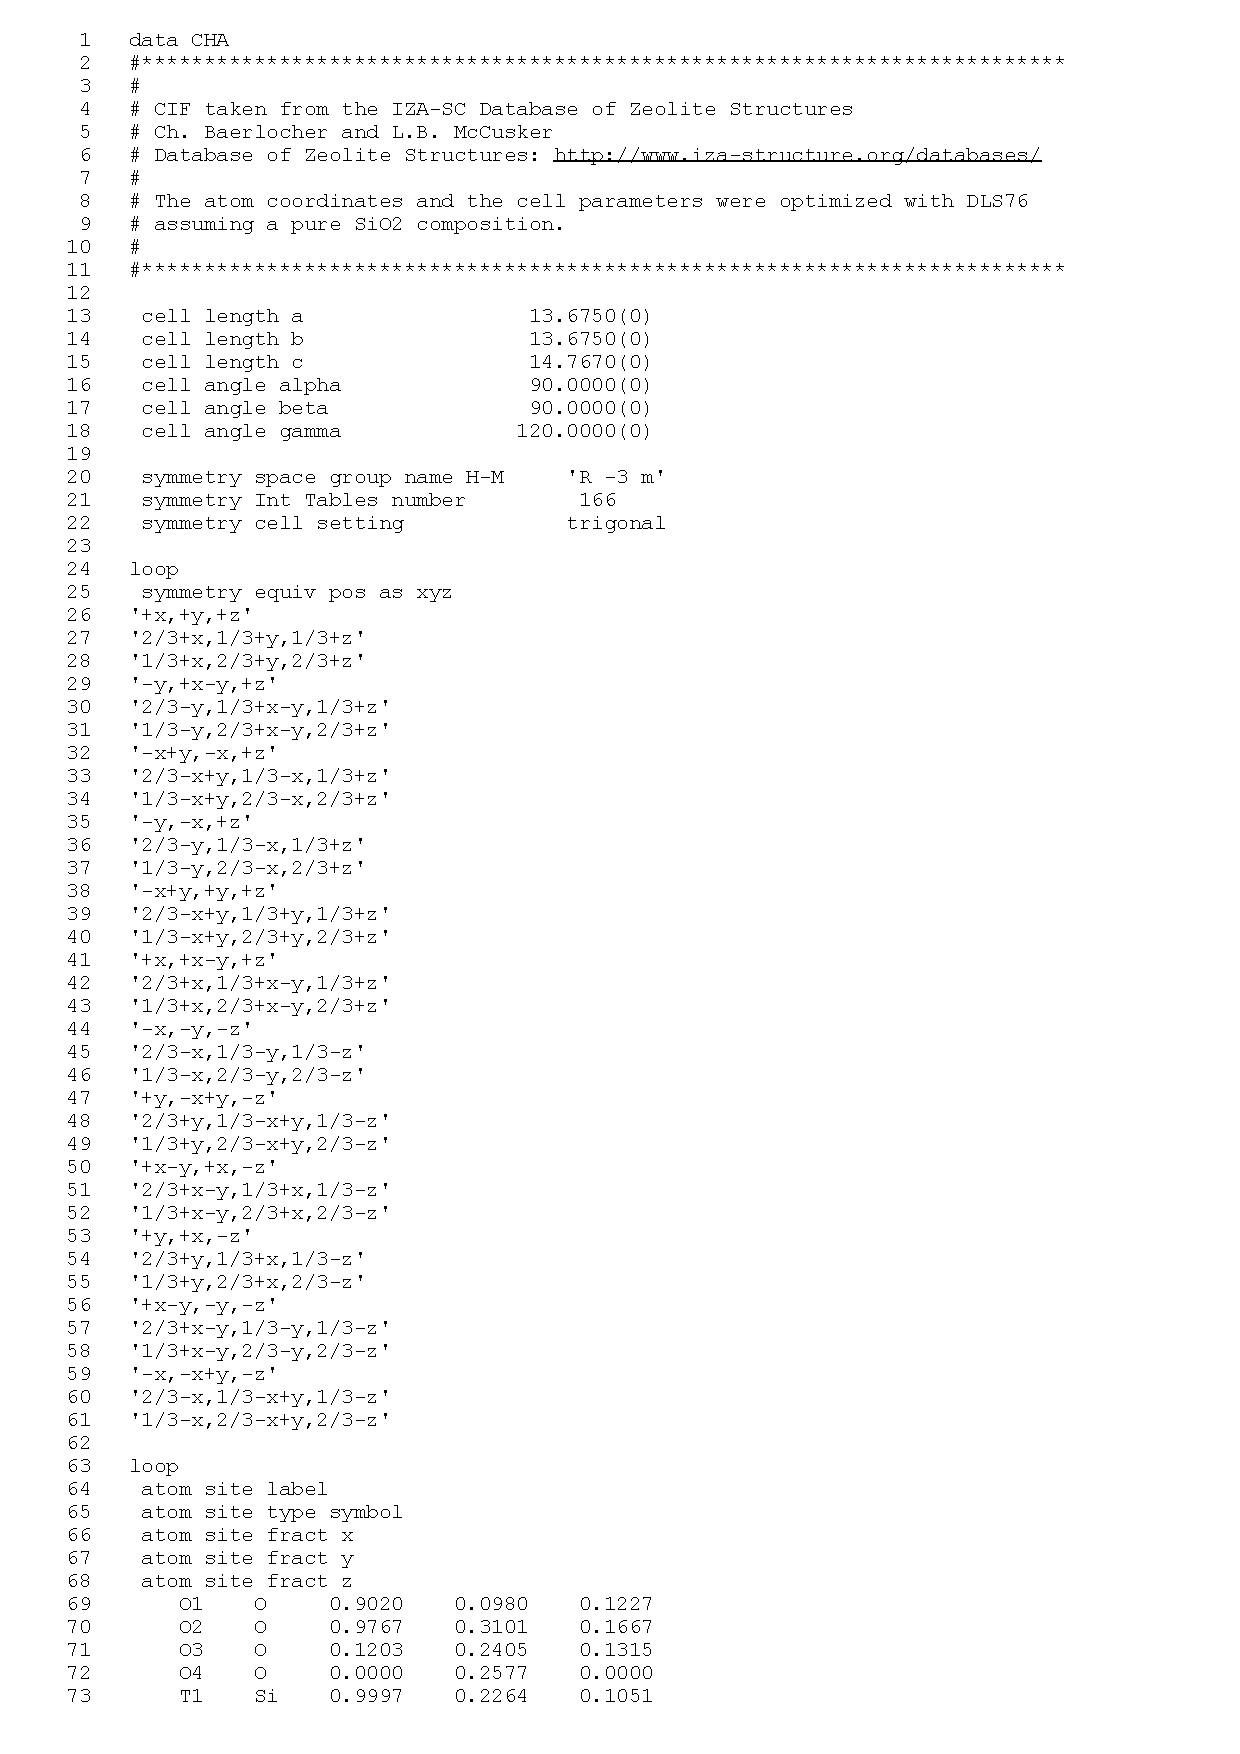
\includepdf[pages=-]{Bijlages/Bijlage_B.pdf}

\chapter*{Bijlage E}
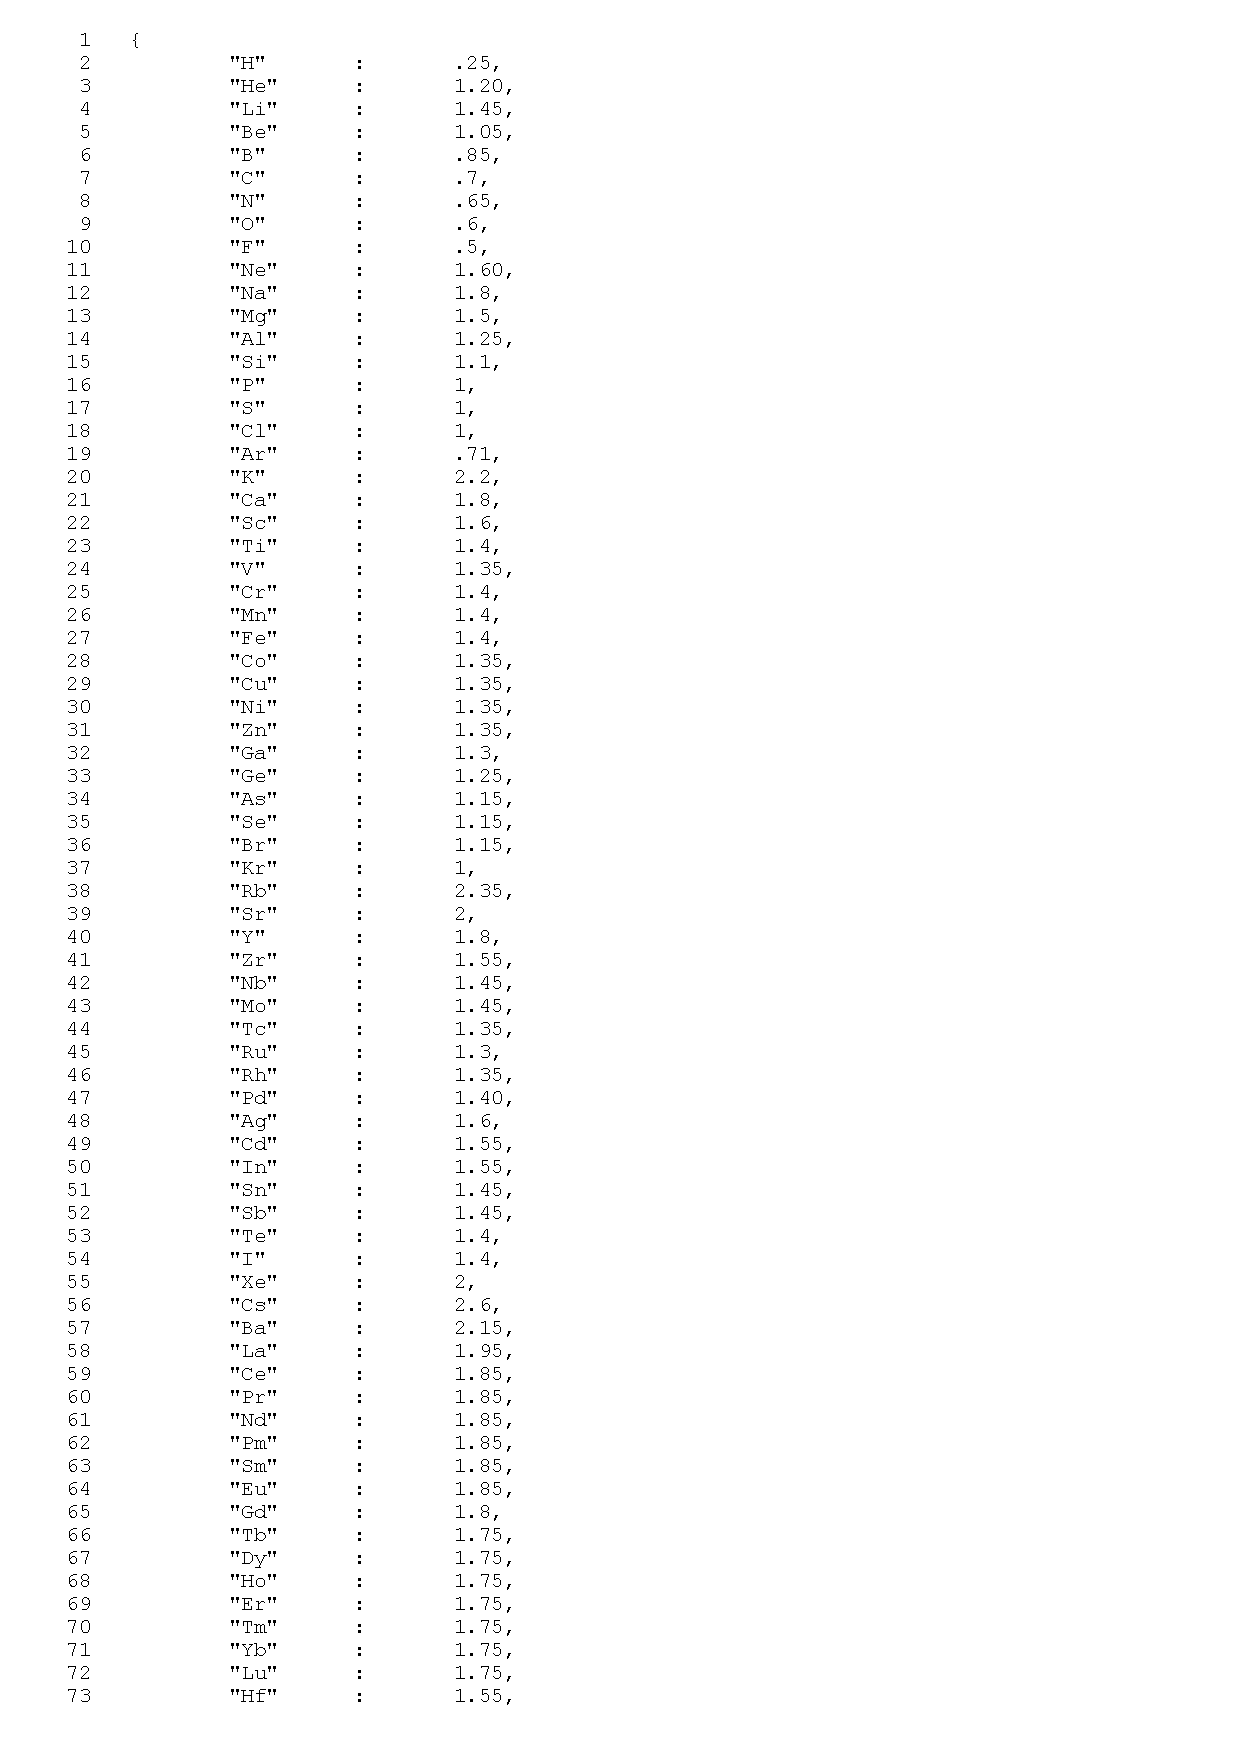
\includepdf[pages=-]{Bijlages/Bijlage_E.pdf}

\chapter*{Bijlage F}
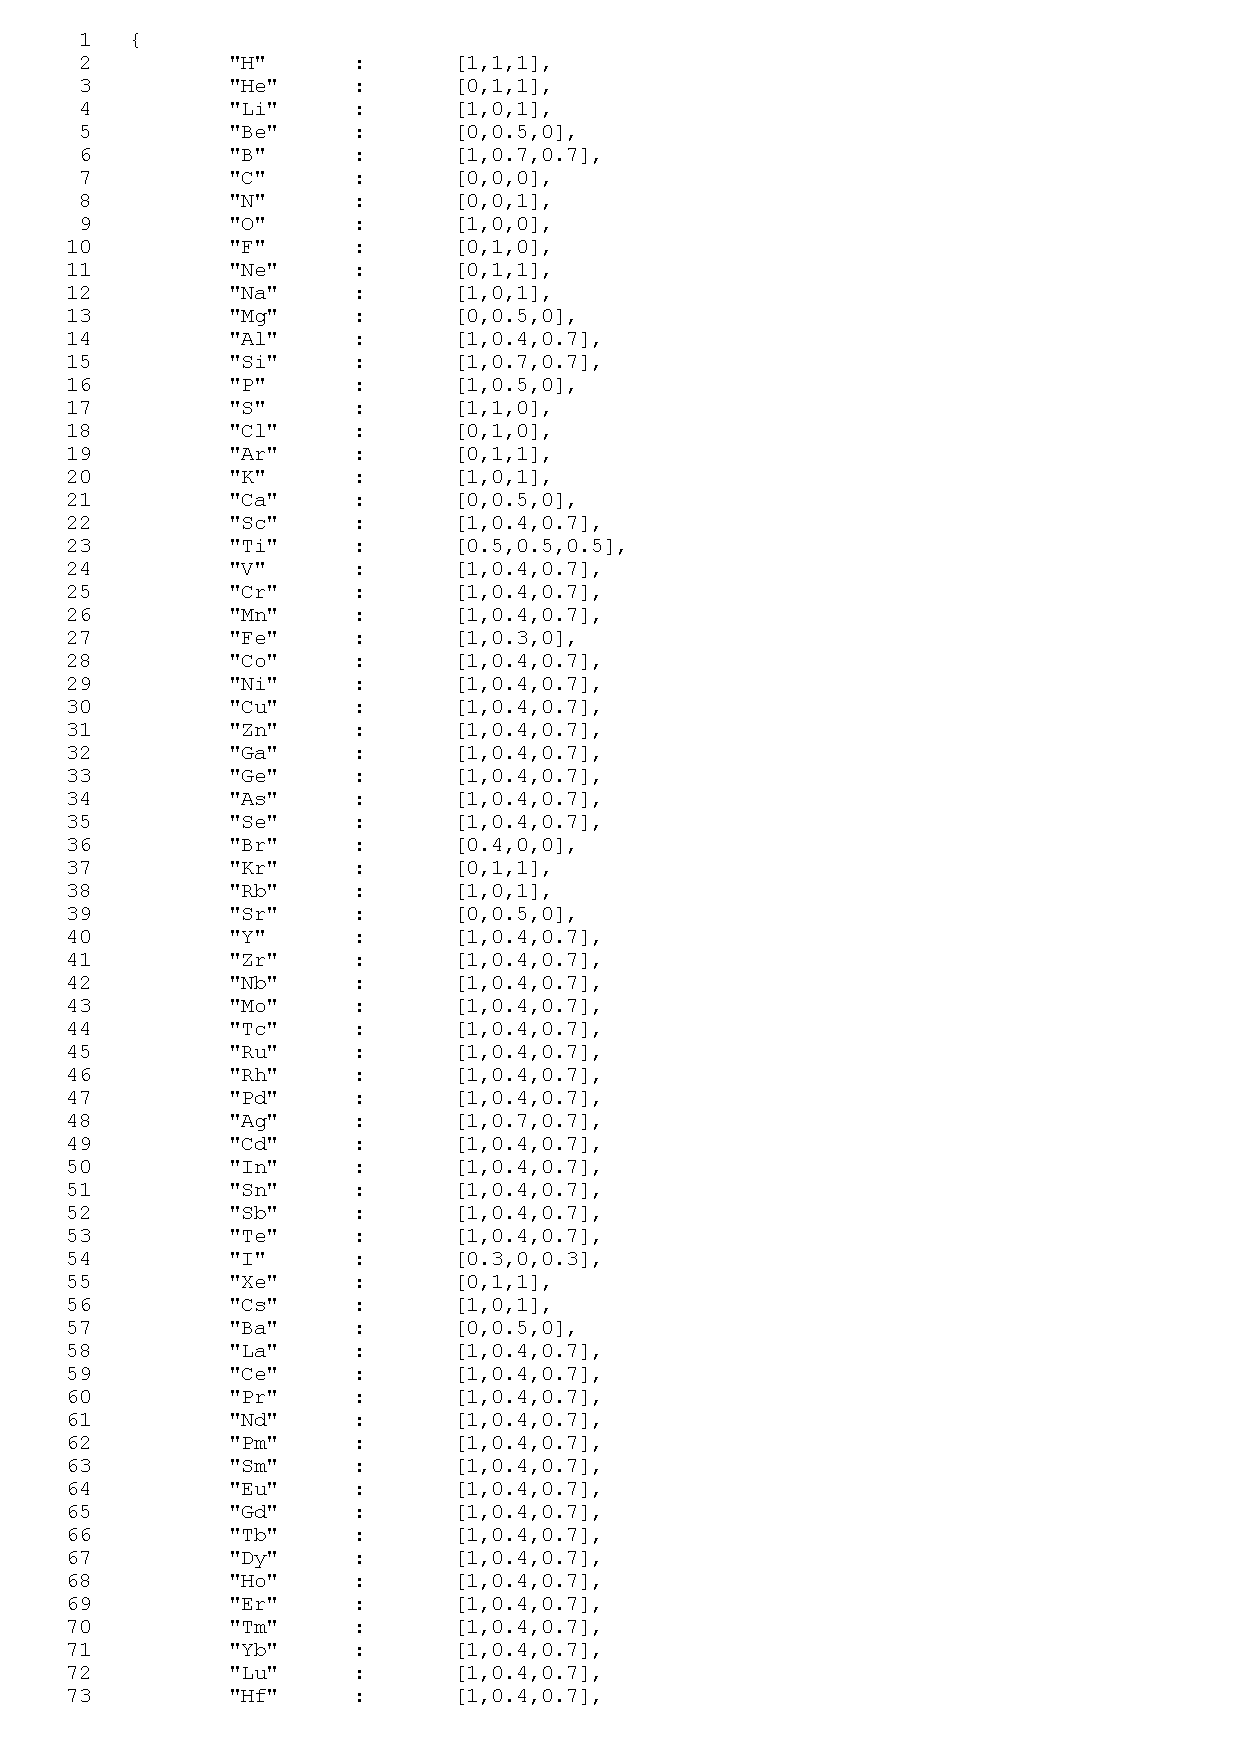
\includepdf[pages=-]{Bijlages/Bijlage_F.pdf}

\chapter*{Bijlage G}
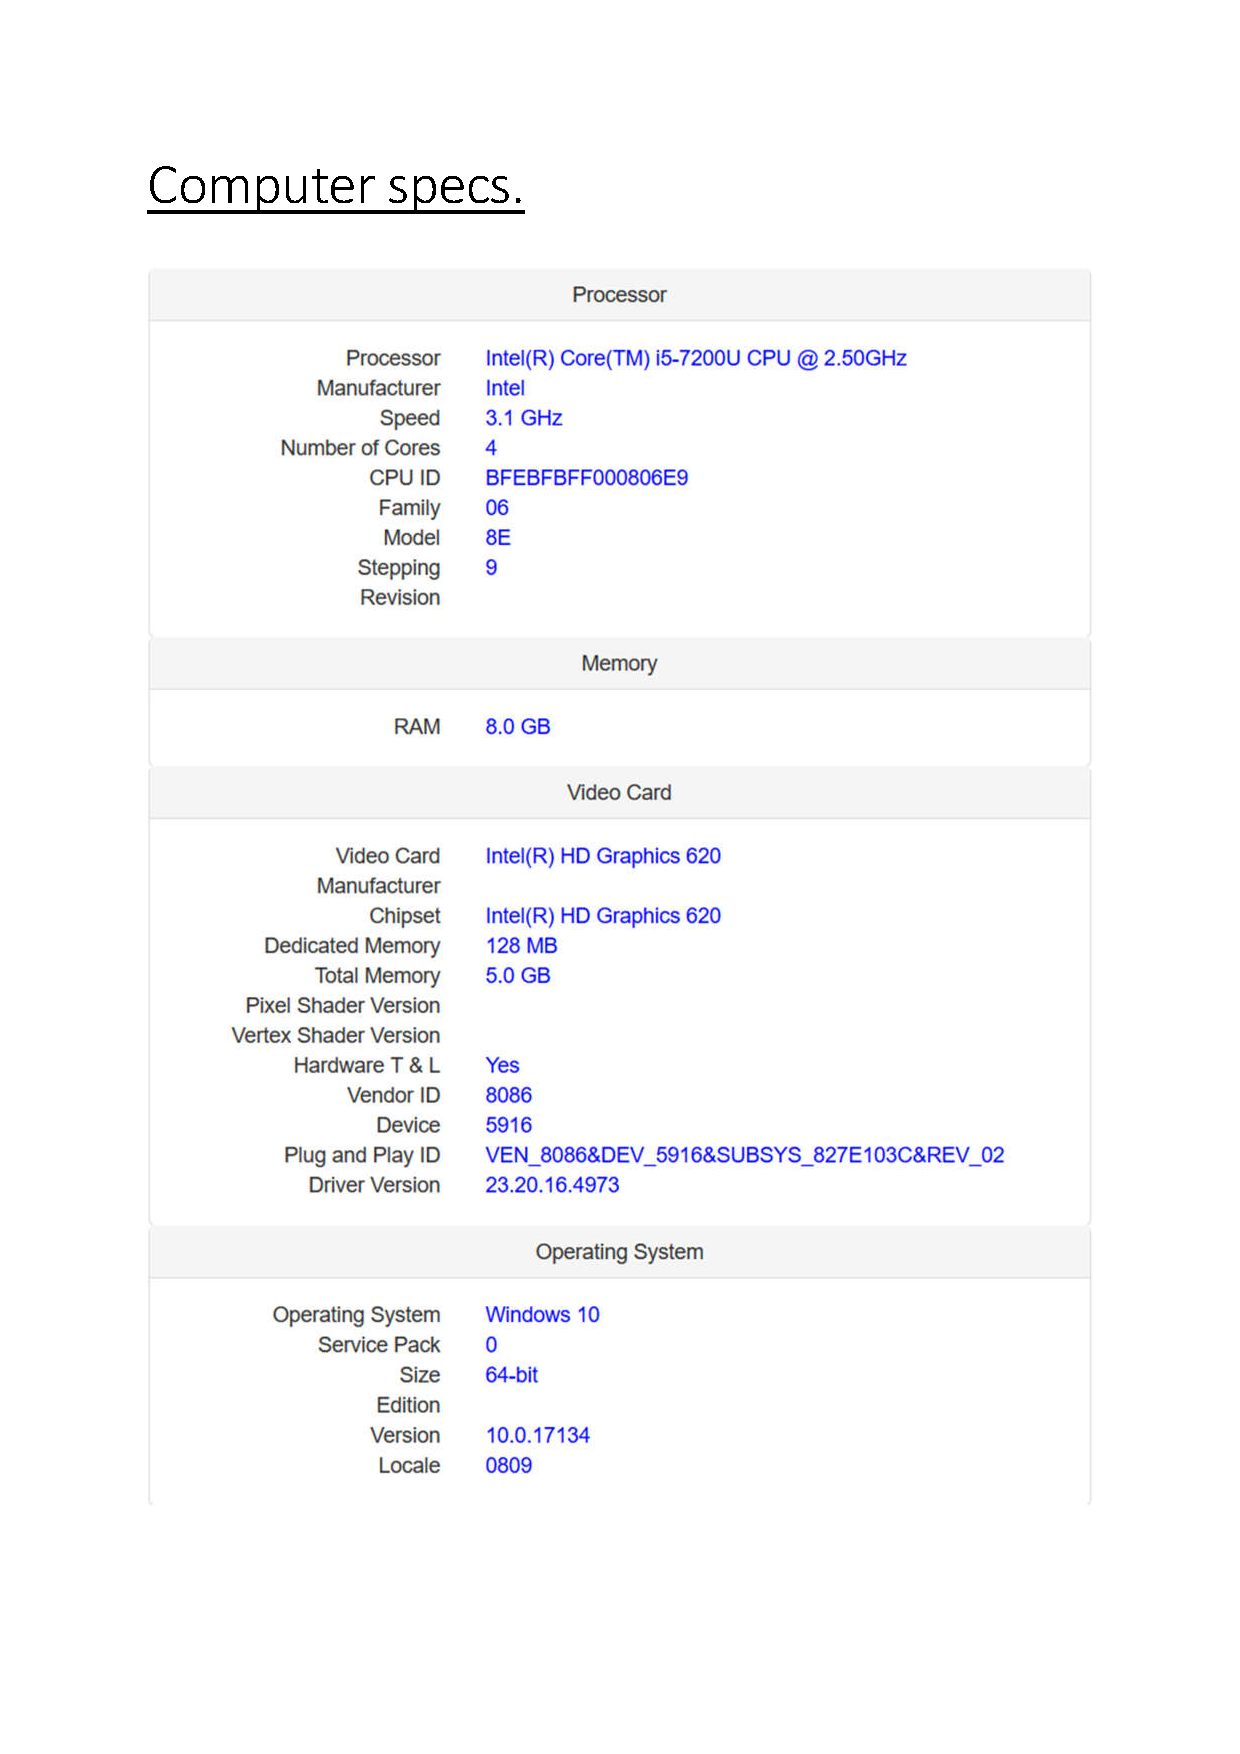
\includepdf[pages=-]{Bijlages/Bijlage_G.pdf}
